\documentclass[11pt,a4paper]{article}
\usepackage[UTF8]{ctex}
\usepackage[a4paper,left=25mm,right=25mm,top=22mm,bottom=22mm]{geometry}
\usepackage{fontspec,xeCJK,graphicx,booktabs,tabularx,array,amsmath,amssymb}
\usepackage[hidelinks]{hyperref}
\setmainfont{Times New Roman}
\setCJKmainfont{SimSun}[BoldFont=SimHei]
\setCJKsansfont{SimHei}
\setlength{\parindent}{2em}
\setlength{\parskip}{3pt}
\linespread{1.18}
\setlength{\tabcolsep}{5pt}
\emergencystretch=1em
\pagestyle{plain}
\begin{document}
\section*{1 问题背景}
华北山区的低温与地形条件限制了耕地的种植季数和作物选择，大棚虽能拓展生产时段，其面积和适种范围仍有限。与此同时，作物产得多未必卖得好，集中种植收益较高的品种又可能增加滞销风险，并与轮作和田间管理要求发生冲突。因此，乡村种植安排需要协调土地利用、作物接续与市场承接能力，在有限耕地上形成兼顾生产效益、持续耕作和风险承受能力的多年种植方案。\par
\section*{2 问题重述}
\subsection*{2.1 研究对象与共同条件}
研究对象为某乡村的露天耕地和种植大棚，规划期为2024—2030年。露天耕地共1201亩，分为34个地块；另有16个普通大棚和4个智慧大棚，每个大棚面积均为0.6亩。附件1提供地块和作物的基本情况，附件2提供2023年种植记录及亩产量、种植成本和销售价格等统计资料。不同地类的种植制度见表1。\par
\par\smallskip\noindent\begin{minipage}{\linewidth}
{\centering\small 表1 各类土地的种植制度\par}\smallskip
{\fontsize{10.5}{14}\selectfont\renewcommand{\arraystretch}{1.22}\begin{tabularx}{\linewidth}{>{\raggedright\arraybackslash}p{2.7cm}>{\raggedright\arraybackslash}p{2.4cm}>{\raggedright\arraybackslash}X}\toprule
土地类型 & 年度种植安排 & 作物范围与例外 \\
\midrule
平旱地、梯田、山坡地 & 单季 & 粮食类作物，水稻除外 \\
水浇地 & 单季或两季 & 单季水稻，或两季蔬菜；蔬菜第一季排除大白菜、白萝卜和红萝卜，第二季仅选这三种中的一种 \\
普通大棚 & 两季 & 第一季为蔬菜，排除上述三种；第二季为食用菌 \\
智慧大棚 & 两季 & 两季均为蔬菜，排除上述三种 \\
\bottomrule\end{tabularx}}\end{minipage}\par\smallskip
{\small\noindent 注：上述三种蔬菜仅在水浇地第二季种植，食用菌仅在普通大棚秋冬季种植。各类设施的季次对应月份按附件1执行。\par}\medskip
同一地块每季可合种不同作物，但应遵守表1的专门限制；同一种作物不得在同一地块连续重茬。从2023年起，每个地块及大棚的所有土地三年内至少种植一次豆类。种植方案还应便于耕作与田间管理，避免同种作物的种植地过于分散，以及单个地块内种植面积过小。\par
\subsection*{2.2 三个问题的任务与输出}
\textbf{问题1：稳定条件下的种植安排。} 假定预期销售量、亩产量、种植成本和销售价格相对2023年保持稳定，作物在当季销售。同种作物每季总产量超过相应预期销售量时，分别考虑超额部分滞销浪费、按2023年销售价格的50\%出售两种情形，给出各自的七年最优种植方案，填入 \texttt{result1\_1.xlsx} 和 \texttt{result1\_2.xlsx}。\par
\textbf{问题2：不确定条件下的种植安排。} 在表2给出的变化条件下，综合考虑预期销售量、亩产量、种植成本、销售价格的不确定性及潜在种植风险，给出2024—2030年的最优种植方案，填入 \texttt{result2.xlsx}。\par
\par\smallskip\noindent\begin{minipage}{\linewidth}
{\centering\small 表2 问题2给定的未来变化条件\par}\smallskip
{\fontsize{10.5}{14}\selectfont\renewcommand{\arraystretch}{1.22}\begin{tabularx}{\linewidth}{>{\raggedright\arraybackslash}p{4.3cm}>{\raggedright\arraybackslash}X}\toprule
影响因素 & 题目给定条件 \\
\midrule
小麦、玉米预期销售量 & 有增长趋势，平均年增长率为5\%—10\% \\
其他作物预期销售量 & 每年相对2023年约有±5\%的变化 \\
亩产量 & 受气候等因素影响，每年约有±10\%的变化 \\
种植成本 & 平均每年增长约5\% \\
粮食类销售价格 & 基本稳定 \\
蔬菜类销售价格 & 平均每年增长约5\% \\
食用菌销售价格 & 大约每年下降1\%—5\%，其中羊肚菌每年下降5\% \\
\bottomrule\end{tabularx}}\end{minipage}\par\smallskip
\textbf{问题3：关联条件下的种植策略。} 在问题2的基础上，加入作物间的可替代性和互补性，以及预期销售量与销售价格、种植成本之间的相关性，通过模拟数据求解七年最优种植策略，并与问题2的结果比较分析。\par
三份指定结果表均按年度、地块、季次和作物填写种植亩数，单季作物填在第一季对应位置，保持模板形式不变。问题3另外给出策略及比较分析，题目未指定单独的结果模板。\par
\section*{3 问题分析}
\subsection*{3.1 问题1：协调跨期种植与有限销售能力}
土地配置同时受到空间差异和作物接续的约束。不同地类的可种作物与季数不同，一年的种植选择还会影响下一茬作物及三年内的豆类安排。仅按当年亩收益排序，可能占用其他作物不可替代的适种空间，或使后续轮作难以满足。因此，模型需要同时描述地块、作物、季次和年份之间的适配关系，把2023年种植历史接入规划期，并表达跨期轮作和土地覆盖。合种条件下，豆类累计面积相同也可能对应不同的实际覆盖范围；轮作表达应落实到题目要求的所有土地，而具体空间与接续口径应有一致定义。\par
生产规模的经济价值取决于市场能够正常承接多少产品。同一种作物由多块地共同供给，正常销售上限应在相应销售季统一核算，若逐地块各设一个完整上限，就会放大市场容量。超过上限后，新增产量在两种处置规则下分别不产生收入或仅获得半价收入，种植成本则已经发生。模型因此需要把面积与亩产形成的产量、正常销售量和超额部分分开，按规则计算收入后扣除全部种植成本。附件中的种植面积与亩产资料反映生产能力，并不直接给出预期销售量；正常销售上限与价格区间的代表值应分别说明取值依据。\par
可实施的方案还要控制种植安排的细碎程度。允许合种有助于利用土地，却也可能将同一作物分到许多地块，或产生过小的种植片区；仅追求账面收益会遗漏这些管理负担。因此，模型需要在经济收益与布局可管理性之间建立明确的约束或评价联系。“分散”与“小面积”的量化应符合地块尺度和可得信息，地块数量本身也不等同于实际交通距离或作业成本。\par
\subsection*{3.2 问题2：把未来变化转化为当前决策的风险}
未来条件的变化具有不同的时间结构。小麦、玉米销量的增长趋势与其他作物相对2023年的波动含义不同，成本和各类价格也各有变化方向。如果对所有因素逐年套用同一种涨跌方式，就会改变题目给定的基准关系。模型需要区分长期趋势、年度扰动及其作用对象，在统一时间口径下形成未来参数；各类大棚与水浇地季次对应的月份不同，还要求生产、销售和年度参数在时间上相互匹配。题目给出的范围并未规定各取值的发生概率，概率与共同变化方式属于建模设定。\par
风险来自种植安排与未来市场、产出之间的错配。播种后，减产可能削减可售产品，需求不足可能使产品转入低价或滞销部分，成本上涨则会直接压缩利润；这些因素同时出现时，方案表现可能比单项变化更差。将未来参数各取一个中间值，只能描述一个代表条件，难以反映不利情况下的损失。因此，模型需要在多种可能条件下评价同一方案，同时考察收益水平和不利表现，并明确二者如何影响种植选择。Q2的超额处置办法及折价基准应单独界定，以保持每种未来条件下的收入含义一致。\par
方案的可实现性还取决于决策时能掌握哪些信息。为每种未来情况分别安排最有利的种植方案，再汇总其收益，相当于预先知道了未来；实际经营者必须在相应信息到来之前作出部分决定。因此，模型需要说明七年计划是一次制定还是允许逐年调整，并限定调整时可用的信息。这样才能区分可实施策略与事后看来最有利的安排，使风险评价对应真实的决策处境。\par
\subsection*{3.3 问题3：区分作物间相互作用与共同变化}
作物间的替代、互补关系与经济变量的相关性具有不同含义。替代或互补涉及一种产品的市场条件变化如何影响另一种产品的需求或配置价值；相关性描述多个量是否共同变化。例如，两种蔬菜销量同时上升，可能是共同季节需求所致，单凭同向变化不足以确认互补关系。因此，模型需要分别表达作物间的作用关系与销量、价格、成本的联合变化，并说明关系的对象、方向和强度。两类机制若使用相同影响来源，还应避免重复计入；具体关系形式与参数依据应与可取得的资料相匹配。\par
问题3的比较应辨明，考虑关系后种植策略及其收益、风险究竟发生了什么变化。若两问同时采用不同的销量基准、销售规则或未来条件，观察到的差异就混合了多种影响。因而，模型需要将Q2方案与加入关系后的方案置于一致的比较口径下，并考察关系设定改变时判断是否随之变化。原附件提供的是2023年种植记录和根据近年资料形成的统计摘要，并非直接给出的多年联合观测序列；由假设关系生成的模拟结果仅支持相应设定下的策略比较，不等同于已经识别了当地真实关系，也不预设增加关系后必然获得更高收益。\par
\section*{4 总体思路}
三问共享土地、作物、季次和年份构成的种植对象，以及农业约束和产量—销售—收益核算关系。为说明每问改变的是哪些组成部分，将这一共同结构及任务增量整理为图1。\par
\par\noindent\hfil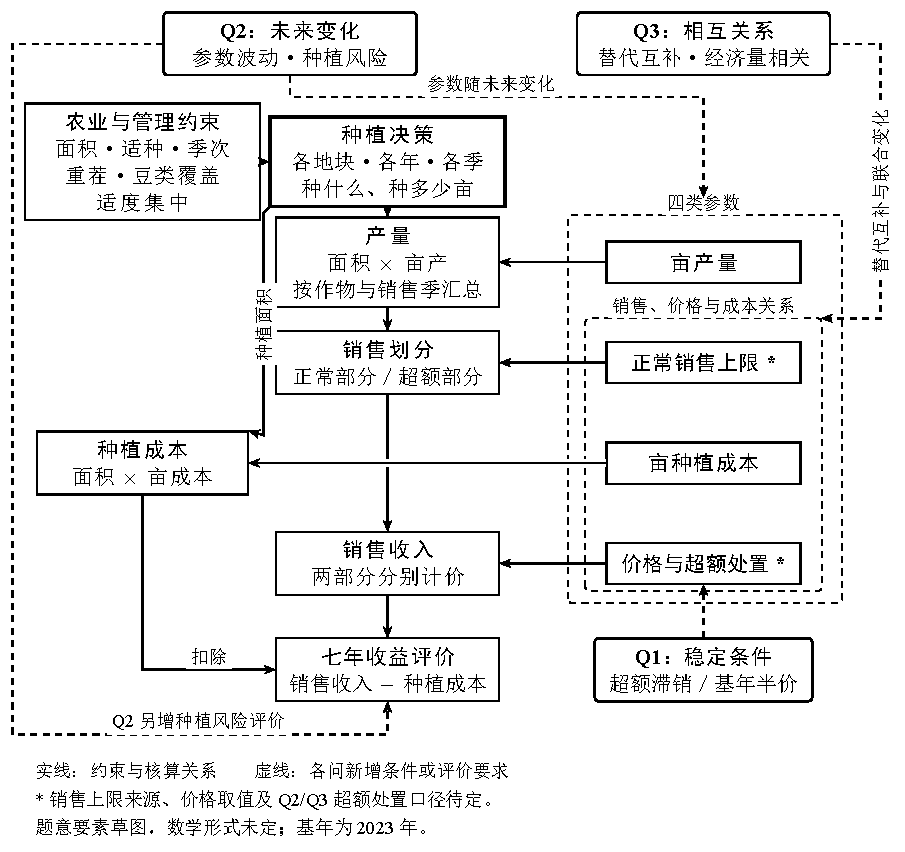
\includegraphics[width=0.96\linewidth]{../figures/understanding_v2/render_v2/framework.pdf}\hfil\par\nopagebreak
{\centering\small 图1 统一种植决策与三问扩展的模型框架（建模要素草图）\par}\medskip
Q1在稳定条件下分别处理两种超额销售规则；Q2加入未来参数变化与种植风险；Q3进一步引入作物关系和经济变量相关性，并以Q2方案为比较基准。三问的递进发生在条件与关系表达上，后问的种植面积仍可重新选择。\par
据此，后文先明确共同输入和农业规则，再依次展开稳定条件、不确定条件与关联条件下的种植决策。图示表达题意支持的要素与作用关系，具体数学形式随各问研究确定。\par
\par\vspace{8pt}\noindent\begin{minipage}{\linewidth}
\section*{5 符号说明框架}
为便于统一描述各小问，先列出题意阶段已确定的公共对象、时间与资源符号。\par
\par\smallskip\noindent\begin{minipage}{\linewidth}
{\fontsize{10.5}{14}\selectfont\renewcommand{\arraystretch}{1.22}\begin{tabularx}{\linewidth}{>{\raggedright\arraybackslash}p{2.2cm}>{\raggedright\arraybackslash}X>{\raggedright\arraybackslash}p{4.6cm}}\toprule
符号 & 含义 & 单位或范围 \\
\midrule
$I$，$i$ & 地块集合及其索引，包含露天耕地和大棚 & 以附件1的地块标识为准 \\
$J$，$j$ & 作物集合及其索引 & 以附件1的作物编号为准 \\
$T$，$t$ & 规划年份集合及其索引 & $T=\{2024,\ldots,2030\}$ \\
$t_0$ & 历史基准年 & $t_0=2023$ \\
$A_i$ & 地块 $i$ 的可用耕地面积 & 亩 \\
\bottomrule\end{tabularx}}\end{minipage}\par\smallskip
\end{minipage}
\end{document}
